\documentclass[final]{siamltex}
%test change
\usepackage{cite}
\usepackage{graphicx,bbm,pstricks,soul}
\usepackage{pifont}
\usepackage{bbm,algorithmic,mdframed,placeins,multirow,booktabs,subfigure}
\usepackage[ruled,vlined,linesnumbered]{algorithm2e}
\usepackage{tikz,hhline}
\usepackage{tabularx}
\newcolumntype{L}[1]{>{\raggedright\let\newline\\\arraybackslash\hspace{0pt}}m{#1}}
\newcolumntype{C}[1]{>{\centering\let\newline\\\arraybackslash\hspace{0pt}}m{#1}}
\newcolumntype{R}[1]{>{\raggedleft\let\newline\\\arraybackslash\hspace{0pt}}m{#1}}

\setlength{\parindent}{0in}
\usepackage{amsmath,amsfonts,amsbsy,amssymb}
\newcommand{\RARR}[3]{#1
  \;\displaystyle\mathop{\displaystyle\longrightarrow}^{#3}\; #2}
\newcommand{\RARRlong}[3]{#1
  \;\displaystyle\mathop{-\!\!\!-\!\!\!-\!\!\!-\!\!\!-\!\!\!\!\displaystyle
  \longrightarrow}^{#3}\; #2}
\newcommand{\LARR}[3]{#1
  \;\displaystyle\mathop{\displaystyle\longleftarrow}^{#3}\; #2}
\newcommand{\LRARR}[4]{{\mbox{ \raise 0.4 mm \hbox{$#1$}}} \;
  \mathop{\stackrel{\displaystyle\longrightarrow}\longleftarrow}^{#3}_{#4}
  \; {\mbox{\raise 0.4 mm\hbox{$#2$}}}}
\newcommand{\bX}{{\bf X}}
\newcommand{\vecx}{{\mathbf x}}
\newcommand{\vecy}{{\mathbf y}}
\newcommand{\vecz}{{\mathbf z}}
\newcommand{\vecq}{{\mathbf q}}
\newcommand{\bs}{{\mathbf s}}
\newcommand{\vecr}{{\mathbf r}}
\newcommand{\vecX}{{\mathbf X}}
\newcommand{\vecv}{{\mathbf v}}
\newcommand{\tick}{\ding{52}}
\newcommand{\cross}{\ding{54}}
\newcommand{\vecn}{{\mathbf n}}
\newcommand{\vecp}{{\mathbf p}}
\newcommand{\cT}{{\mathcal T}}
\newcommand{\dt}{{\mbox{d}t}}
\newcommand{\dx}{{\mbox{d} \vecx}}
\newcommand{\boldnu}{{\boldsymbol \nu}}
\newcommand{\er}{{\mathbb R}}
\renewcommand{\div}{{\rm div}}
\newcommand{\bnu}{{\bf \nu}}
\newcommand{\divergence}{\mathop{\mbox{div}}}
\renewcommand{\P}{\mathbb{P}}
\newcommand{\FP}{P_{\rm{FP}}}
\newcommand{\ME}{P_{\rm{ME}}}
\newcommand{\MEs}{P_{\rm{ME}_{S}}}
\newcommand{\D}{\mathcal{D}}
\newcommand{\G}{\mathcal{G}}
\newcommand{\N}{\mathcal{N}}
\newcommand{\X}{{\mathbf X}}
\newcommand{\Y}{{\mathbf Y}}
\newcommand{\W}{{\mathbf W}}
\newcommand{\data}{D}
\newcommand{\neff}{n_{\text{eff}}}
\newcommand{\E}{{\mathbb E}}
\renewcommand{\b}[1]{{\bf #1}}
\DeclareMathOperator*{\argmin}{arg\,min}
\DeclareMathOperator*{\argmax}{arg\,max}

\newcommand{\picturesAB}[6]{
\centerline{
\hskip #4
\raise #3 \hbox{\raise 0.9mm \hbox{(a)}}
\hskip #5
\epsfig{file=#1,height=#3}
\hskip #6
\raise #3 \hbox{\raise 0.9mm \hbox{(b)}}
\hskip #5
\epsfig{file=#2,height=#3}
}}
\newcommand{\picturesCD}[6]{
\centerline{
\hskip #4
\raise #3 \hbox{\raise 0.9mm \hbox{(c)}}
\hskip #5
\epsfig{file=#1,height=#3}
\hskip #6
\raise #3 \hbox{\raise 0.9mm \hbox{(d)}}
\hskip #5
\epsfig{file=#2,height=#3}
}}

\makeatletter  
\newcommand{\xleftrightarrows}[2][]{\mathrel{%  
 \raise.40ex\hbox{$  
       \ext@arrow 3095\leftarrowfill@{\phantom{#1}}{#2}$}%  
 \setbox0=\hbox{$\ext@arrow 0359\rightarrowfill@{#1}{\phantom{#2}}$}%  
 \kern-\wd0 \lower.4ex\box0}}  
 
\newcommand{\xrightleftarrows}[2][]{\mathrel{%  
 \raise.40ex\hbox{$\ext@arrow 3095\rightarrowfill@{\phantom{#1}}{#2}$}%  
 \setbox0=\hbox{$\ext@arrow 0359\leftarrowfill@{#1}{\phantom{#2}}$}%  
 \kern-\wd0 \lower.4ex\box0}}  
 
\def\leftrightarrowfill@{%
 \arrowfill@\leftarrow\relbar\rightarrow%
 }
\newcommand*{\centerfloat}{%
  \parindent \z@
  \leftskip \z@ \@plus 1fil \@minus \textwidth
  \rightskip\leftskip
  \parfillskip \z@skip}
\makeatother
\makeatother 

\newcommand\irregularcircle[2]{% radius, irregularity
  \pgfextra {\pgfmathsetmacro\len{(#1)+rand*(#2)}}
  +(0:\len pt)
  \foreach \a in {10,20,...,350}{
    \pgfextra {\pgfmathsetmacro\len{(#1)+rand*(#2)}}
    -- +(\a:\len pt)
  } -- cycle
}

\newcommand{\into}{\operatornamewithlimits{\longrightarrow}}
\newtheorem{dfn}{Definition}[section]

\newcommand{\ltri}{%
\,\resizebox{!}{0.25\baselineskip}{%
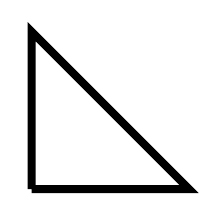
\begin{tikzpicture}%
\draw[line width=1mm](0,0) -- (0,2) -- (2,0)  -- (0,0);
\end{tikzpicture}%  
}\xspace%
}%

\newcommand{\smallltri}{%
\,\resizebox{!}{0.15\baselineskip}{%
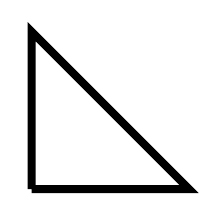
\begin{tikzpicture}%
\draw[line width=1mm](0,0) -- (0,2) -- (2,0)  -- (0,0);
\end{tikzpicture}%  
}\xspace%
}%

\title{Transport map accelerated-PAIS, and application to inverse problems arising from
  multiscale stochastic reaction networks}
\author{Simon Cotter, Yannis Kevrekidis, Paul Russell}
\begin{document}
\maketitle
\begin{abstract}
In many applications, inverse problems arise where where there are
complex correlations between the different parameters which we wish to
infer from data. The correlations often manifest themselves as lower
dimensional manifolds on which the likelihood function is
invariant, or varies very little. This can be due to trying to infer
unobservable parameters, or due to sloppiness in the model which is
being used to describe the data. In such a situation, standard
sampling methods for characterising the posterior distribution which
do not incorporate information about this structure will be highly
inefficient. Moreover, most methods are inherently serial in nature,
and as such are not expoiting the parallelised  nature of modern
computer infrastructure. In this paper, we seek to develop a method to
tackle this problem, using optimal transport maps to simplify
posterior distributions which are concentrated on lower dimensional
manifolds.

We demonstrate the approach by considering inverse problems arising
from partially observed stochastic reaction networks. In particular,
we consider systems which exhibit multiscale behaviour, but for which
only the slow variables in the system are observable. We demonstrate
that certain multiscale approximations lead to more consistent
approximations of the posterior than others.
\end{abstract}


\section{Introduction}
%Topics to cover: parallel MCMC, pMC, PAIS
%Transport maps, transport map MCMC
%Stochastic reaction networks
%Multiscale approximations, QSSA/QEA, CMA

In Section \ref{sec:map} we show how an appropriate transport map can
be constructed from importance samples which maps the posterior close
to a reference Gaussian measure. In Section \ref{sec:TPAIS} we show
how such a map can be incorporated into a sophisticated parallel MCMC
infrastructure in order to accelerate mixing. In Section
\ref{sec:multi} we consider how likelihoods can be approximated using
multiscale methodologies in order to carry out inference for
multiscale and/or partially observed stochastic reaction networks. In
Section \ref{sec:num} we present some numerical examples, which serve
to demonstrate the increased efficiency of the described sampling
methodologies, as well as investigating the posterior approximations
discussed in the previous section. We conclude with a discussion in
Section \ref{sec:conc}.

\section{Construction of transport maps in importance sampling} \label{sec:map}
%Follow the other papers, show adaptation(s)

In this section, we give details on how we have adapted the method
proposed in \cite{parno2014transport} to couple the target,
$\mu_{\theta}$, with the reference distribution, $\mu_r$. In many
applications ***REFS*** inverse problems arise which lead to posterior
distributions from which it is challenging to sample efficiently. This
can be due to multimodality, strong correlations between parameters,
or vastly different scales of sensitivity in different directions, for
example the concept of sloppy models. Standard random walks become
inefficient in this context since the proposal distributions do not
take into account these types of challenging structures in the
density, leading to a large number of proposals being made in low
density regions.

One way that this can be tackled is to implement more complex MCMC
methods which are able to explore the state space more
efficiently. For example the Metropolis-Adjusted Langevin Algorithm (MALA) or Hamiltonian Monte
Carlo (HMC) methods use gradient information about the target density
in order to make proposals in better directions that RWMH. Riemannian
manifold MCMC methods can use additionally approximations of the
Hessian of the target in order to make very large moves with a good
probability of being accepted.

Another approach is the simplification of the posterior density
itself. In \cite{parno2014transport}, the authors proposed the
approximation of an invertible map which exactly couples the postieror distribution
$\mu_{\theta}$ to a reference measure $\mu_r$. Given such a map,
$T\in\mathcal{T}$, $T\colon \mathcal{X}\rightarrow\mathbb{R}^d$, we can then draw a proposal sample from $\pi_r$, before mapping these samples back onto target space using $T^{-1}$. These proposed samples are distributed according to the target distribution. On target space, the proposal distribution is induced by the pullback of the standard Gaussian through the map,
\begin{equation}\label{eq:pullback}
	\tilde{\pi}(\theta) = \pi_r(T(\theta))|J_T(\theta)|,
\end{equation}
which is equal to the target density when $T$ is exact. Clearly we
require $T$ to be monotonic and have continuous first derivatives,
which means that our space of feasible transference plans,
$\mathcal{T}^\uparrow$, may not include the exact map. Since it is
unlikely that $T\in\mathcal{T}^\uparrow$, we are motivated to
formulate an optimisation problem as discussed in
Section~\ref{sec:intro_optim}.  ****PAUL, what is
$\mathcal{T}^\uparrow$, what is in Section~\ref{sec:intro_optim}*****

We attempt to find a deterministic coupling of two continuous probability distributions, $(\mu_\theta, \mu_r)$, such that $\mu_r = T\mu_\theta$ is satisfied and also that $T \in \mathcal{T}^\uparrow$. There may be infinitely many such couplings, so we look to find the coupling which minimises the difference between the proposal density and the target distribution, i.e. the distance between $\pi(\theta)$ and $\tilde{\pi}(\theta)$. In this case, we measure this distance using the Kullback-Leibler divergence.

The map does not necessarily satisfy the monotonicity condition when we optimise the cost function,
\[
	C(T) = D_\text{KL}(\pi\|\tilde{\pi}),
\]
so it must be enforced in the design of each map component. To guarantee these properties we carefully choose the basis functions for each component, and we restrict the map to be lower triangular, i.e. $T \in \mathcal{T}^{\ltri}\subset\mathcal{T}^\uparrow$. This lower triangular map has the form,
\[
	T(\theta_1, \dots, \theta_n) = \begin{bmatrix} T_1(\theta_1) \\ T_2(\theta_1, \theta_2) \\ \vdots \\
		T_n(\theta_1, \dots, \theta_n) \end{bmatrix},
\]
where $T_i\colon \mathbb{R}^i \to \mathbb{R}$. We also assume that the target and reference probability densities are absolutely continuous on
$\mathbb{R}^d$ which guarantees the maps existence.

\subsection{The optimisation problem}

With these constraints in mind we formulate the optimisation problem explicitly. The cost function
is chosen to be the Kullback-Leibler divergence between the posterior density and the pullback density,
\[
	D_\text{KL}(\pi\|\tilde{\pi}) =
		\mathbb{E}_\pi\left[\log\left(\frac{\pi(\theta)}{\tilde{\pi}(\theta)}\right)\right].
\]
Given the form of the pullback in Equation~\eqref{eq:pullback}, now taken through an approximate map, the divergence becomes
\[
	D_\text{KL}(\pi\|\tilde{\pi}) = \mathbb{E}_\pi\left[\log\pi(\theta) - \log\pi_r(\tilde{T}(\theta)) -
		\log\left|J_{\tilde{T}}(\theta)\right|\right].
\]
We note the posterior density is constant in $\tilde{T}$, and so it is not necessary for us to compute it when optimising this cost function. This expression is a complicated integral with respect to the target distribution, for which the normalisation constant is unknown, however this is exactly the scenario for which we would turn to MCMC methods for a solution.

To find the best coupling, $\tilde{T} \in \mathcal{T}^{\ltri}$, we solve the optimisation problem,
\[
	\tilde{T} = \arg\min_{T \in \mathcal{T}^{\smallltri}} \mathbb{E}_\pi\left[-\log\pi_r(T(\theta)) -
		\log\left|J_T(\theta)\right|\right]
\]
which has a unique solution. However we would like to ensure that this solution is regular and monotonic. For this
reason we regularise the problem further. The optimisation problem now takes the form
\begin{equation}\label{eq:gen_map_optim}
	\tilde{T} = \arg\min_{T\in\mathcal{T}^{\smallltri}} \left[
		 \mathbb{E}_\pi\left[-\log\pi_r(T(\theta)) -
		\log\left|J_T(\theta)\right|\right] + \beta\mathbb{E}(T(\theta)- \theta)^2 \right].
\end{equation}
This parameter $\beta$ does not need to be tuned, experimentation has shown that the choice
$\beta=1$ is sufficient for most problems. The form of the penalisation term promotes maps which are
close to the identity, and hence are likely to be monotonic.

\subsection{The structure of the map}

Before we continue with the derivation of the optimisation problem, we consider the structure
of the map in more detail. The lower lower triangular structure of the map not only guarantees monotonicity, it also allows for efficient calculation of the pullback density as well as the inverse of the map, $T^{-1}$. The Jacobian of $T$ is a lower triangular matrix,
\[
	DT(\theta) = \begin{bmatrix}
		\partial_{\theta_1} T_1(\theta) & \dots & \partial_{\theta_d} T_1(\theta)\\
		\vdots & \ddots & \vdots \\
		\partial_{\theta_1} T_d(\theta) & \dots & \partial_{\theta_d} T_d(\theta)
	\end{bmatrix} = \begin{bmatrix}
		\partial_{\theta_1} T_1(\theta) & \dots & 0\\
		\vdots & \ddots & \vdots \\
		\partial_{\theta_1} T_d(\theta) & \dots & \partial_{\theta_d} T_d(\theta)
	\end{bmatrix}
\]
since $\partial_{\theta_n} T_k(\theta) = 0$ for all $n > k$. This lower triangular structure means that the determinant of the Jacobian is a product of the diagonal elements which, when we take logs, becomes
\begin{equation}\label{eqn:separable_jacobian}
	\log\left|J_T(\theta)\right| = \sum\limits_{i=1}^d \! \log \partial_{\theta_i} T_i(\theta).
\end{equation}
Here we note that this term is separable in terms of the dimension $i$.

Inverting $T$ is simplified by the lower triangular structure in the sense that each dimension, $i$, we need only invert a univariate polynomial. This simplification comes about because we invert each dimension of the map independently, beginning with $T_1$ which is a function of only $\theta_1$. Finding the root of $T_1(\theta_1) = r_1$, gives us the value of $\theta_1$ which we can then use to find the root of $T_2(\theta_2;\theta_1) = r_2$, and so on. These roots, $r_1,\dots,r_d$, are restricted to be real since $\mathcal{X} \subset \mathbb{R}^d$, which allows us to find the unique point, $\theta$, which corresponds to the point $r$.

We require that the first derivatives of the map are continuous, which is easy to enforce by the choice of basis functions. Here we assume that the map will be built from a family of orthogonal polynomials, $\mathcal{P}(\theta)$, although not necessarily orthogonal with respect to the target distribution. Each component of the map is defined as a multivariate polynomial expansion,
\begin{equation}\label{eq:map_defn}
	\tilde{T}_i(\theta; \gamma_i) = \sum\limits_{\mathbf{j}\in\mathcal{J}_i} \!
\gamma_{i,\mathbf{j}}\psi_\mathbf{j}(\theta).
\end{equation}
The parameter $\gamma_i$ is a vector of coefficients in $\mathbb{R}^{M_i}$. Each component of $\gamma_i$ corresponds to a basis function
$\psi_\mathbf{j}$, indexed by the multi-index $\mathbf{j} \in \mathbb{N}_0^d$, here $d$ is the dimension of
$\theta$. These multi-indices are elements of the multi-index set $\mathcal{J}_i$. A multi-index defines a product of univariate polynomials in $\theta_k$,
\[
	\psi_\mathbf{j}(\theta) = \prod\limits_{k=1}^i \! \varphi_{j_k}(\theta_k), \quad \text{for} \quad \mathbf{j} \in \mathcal{J}_i,
\]
and where $\varphi_{j_k}(\theta_k) \in \mathcal{P}(\theta_k)$. Since $\tilde{T}$ is lower triangular, a multi-index $\mathbf{j}\in\mathcal{J}_i$ only contains entries for univariate polynomials in $\theta_k$ for $k\leq i$.

The cardinalities of the multi-index sets $M_i = \text{card}(\mathcal{J}_i)$ give the number of unknowns in our
optimisation problem, and so we would like to keep this number as small as possible. One option is
to use polynomials of total order $p$,
\[
	\mathcal{J}_i^\text{TO} = \left\{\mathbf{j}:\|\mathbf{j}\|_1 \leq p, j_k = 0\ \forall k > i\right\},
\]
which is optimal in terms of the amount of information captured by the map about the target. The cardinality of $\mathcal{J}_i^\text{TO}$ is $M_i = {i+p \choose p}$ which increases rapidly in $d$ and $p$. Smaller optimisation problems can be produced by constructing subsets of $\mathcal{J}_i^\text{TO}$. These index sets are discussed further
in~\cite{parno2014transport}, here we stick with polynomials of total order $p$ since we work with low dimensional problems with the PAIS algorithm.

\subsection{Implementation of the optimisation problem}\label{sec:transport_implementation}

We now return to Equation~\eqref{eq:gen_map_optim}, and show how this can be efficiently formulated
for level-2 BLAS routines~\cite{choi1992scalapack}. The Monte Carlo estimator of a function is the
sample average of the function evaluated at each sample, i.e.
\begin{align*}
	C(T) &= \mathbb{E}_\pi\left[ -\log\pi_r(T(\theta)) - \log|J_T(\theta)|\right] +
			\beta\mathbb{E}(T(\theta)-\theta)^2 \\
		&\approx \frac{1}{K}\sum\limits_{i=1}^d \! \sum\limits_{k=1}^K \left[-\log\pi_r(T_i(\theta^{(k)})) -
			\log\left|\frac{\partial T_i}{\partial \theta_i}(\theta^{(k)})\right| + \beta(T_i(\theta^{(k)})-\theta^{(k)})^2\right].
\end{align*}
This cost function will create a map from $\pi$ to any reference density $\pi_r$. We now restrict ourselves to a Gaussian reference by explicitly using a standardised Gaussian density. The above expression simplifies to
\begin{equation}\label{eq:gauss_map_optim}
	C(T) = \frac{1}{K}\sum\limits_{i=1}^d \! \sum\limits_{k=1}^K \left[\frac{1}{2}
		T_i^2(\theta^{(k)}) - \log\frac{\partial T_i}{\partial \theta_i}(\theta^{(k)}) +
		\beta(T_i(\theta^{(k)})-\theta^{(k)})^2\right].
\end{equation}
Note that since we assume that the map is monotonic, the derivatives of each component are
non-negative and so we don't need to take the absolute values in the log. In practise it is infeasible to enforce this condition across the whole parameter space. We instead enforce this condition by ensuring that the derivatives are non-negative at each sample point. This means that when we sample away from these support points while in reference space, it is possible to enter a region of space where the map is not monotonic.

We now return to the structure of the map components given in Equation~\eqref{eq:map_defn}. Since the basis functions are
fixed, the optimisation problem in \eqref{eq:gen_map_optim} is really over the map components $\bar{\gamma} = (\gamma_1, \dots,
\gamma_d)$ where $\gamma_i \in \mathbb{R}^{M_i}$. Note that $C(T)$ is the sum of $d$ expectations, and these expectations each only concern one dimension. Therefore we can rewrite \eqref{eq:gen_map_optim} as $d$ separable optimisation problems.
\begin{align}\label{eq:gamma_map_optim}
	&\arg\min_{\gamma_i\in\mathbb{R}^{M_i}} \frac{1}{K}\sum\limits_{k=1}^K
		\left[\frac{1}{2}T_i^2(\theta^{(k)}; \gamma_i) - \log\frac{\partial T_i}{\partial\theta_i}(\theta^{(k)}; \gamma_i) + \beta(T_i(\theta^{(k)};
		\gamma_i)-\theta^{(k)})^2\right], \\
	&\text{subject to} \quad \frac{\partial T_i}{\partial\theta_i}(\theta^{(k)};
		\gamma_i) > 0 \ \text{for all}\ k=1,\dots,K,\ i=1,\dots,n.
		\notag
\end{align}
The sum in Equation~\eqref{eq:map_defn} is really the inner
product between the vector of map coefficients, and the evaluations of the basis function at a
particular $\theta^{(k)}$. This means that if we organise our basis evaluations into two matrices,
$(F_i)_{k,\mathbf{j}} = \psi_\mathbf{j}(\theta^{(k)})$, and $(G_i)_{k,\mathbf{j}} =
\frac{\partial\psi_\mathbf{j}}{\partial\theta_i}(\theta^{(k)})$, for all $\mathbf{j}
\in \mathcal{J}_i^\text{TO}$, and $k = 1,\dots,K$, then we have that $T_i(\theta^{(k)}) = (F_i)_{k\cdot}\gamma_i$ and $\frac{\partial T_i}{\partial \theta_i}(\theta^{(k)}; \gamma_i) = (G_i)_{k\cdot}\gamma_i$, so \eqref{eq:gen_map_optim} becomes
\begin{align}\label{eq:blas_map_optim}
	&\arg\min_{\gamma_i\in\mathbb{R}^{M_i}} \frac{1}{2}(F_i\gamma_i)^\top(F_i\gamma_i) -
		c^\top\log(G_i\gamma_i) + \beta\sum\limits_{k=1}^K \!
		(F_i\gamma_i-\theta^{(k)})^\top(F_i\gamma_i-\theta^{(k)}), \\
	&\text{subject to} \quad G_i\gamma_i > 0. \notag
\end{align}
In this expression, the vector $c$ is a $K\times 1$ vector of ones, and $\log(G_i\gamma_i)$ is to be
evaluated element-wise. As the Monte Carlo simulations advance, new rows can be appended to the
$F_i$ and $G_i$ matrices, and $F_i^\top F_i$ can be efficiently updated via the addition of rank-1 matrices.

The regularisation term in Equation~\ref{eq:blas_map_optim} can be approximated using Parseval's identity,
\[
	\sum\limits_{k=1}^K \! (F_i\gamma_i-\theta^{(k)})^\top(F_i\gamma_i-\theta^{(k)}) \approx
		\int_{\mathbb{R}^n} |T(\theta)-\theta|^2 \text{d}\mu_\theta =
		\sum\limits_{\mathbf{j}\in\mathcal{J}_i^\text{TO}} (\gamma_{i,\mathbf{j}}-\iota_\mathbf{j})^2,
\]
where $\iota$ is the vector of coefficients for the identity map. This is of course only true when
the polynomial family $\mathcal{P}(\theta)$ is chosen to be orthonormal with respect to $\mu_\theta$; however this
approximation accomplishes the goal of efficiently regularising the optimisation problem.

These simplifications result in the efficiently implementable, regularised optimisation problem for
computing the map coefficients,
\begin{align}\label{eq:final_map_optim}
	&\arg\min_{\gamma_i\in\mathbb{R}^{M_i}} \frac{1}{2K}\gamma_i^\top F_i^\top F_i\gamma_i -
		\frac{c^\top}{K}\log(G_i\gamma_i) + \beta\|\gamma_i-\iota\|^2, \\
	&\text{subject to} \quad G_i\gamma_i > 0. \notag
\end{align}
This optimisation problem can be efficiently solved using Newton iterations. It is suggested
in~\cite{parno2014transport} that this method usually converges in around 10-15 iterations, and we
have seen no evidence that this is not a reasonable estimate. When calculating the map several times
during a Monte Carlo run, using previous guesses of the optimal map to seed the Newton algorithm
results in much faster convergence, usually taking only a couple of iterations to satisfy the stopping
criteria.

\subsection{Implementation of the optimisation problem in PAIS}

In the PAIS algorithm, we use weighted samples to approximate the posterior rather than equally weighted samples. Fortunately, the majority of the derivation of a weighted optimisation problem
follows unchanged. We look at the importance sampling Monte Carlo estimate of $C(T)$, compared with
Equation~\eqref{eq:gauss_map_optim},
\[
	C(T) = \frac{1}{\bar{w}}\sum\limits_{i=1}^n \! \sum\limits_{k=1}^K
		w_k\left[\frac{1}{2}T_i^2(\theta^{(k)}) - \log\frac{\partial
		T_i}{\partial\theta_i}(\theta^{(k)}) + \beta(T_i(\theta^{(k)})-\theta^{(k)})^2\right],
\]
here $w_k$ are the weights associated with each sample $\theta^{(k)}$, and $\bar{w}$ is the sum of
all these weights. This necessitates a minor alteration to the optimisation problem in
Equation~\eqref{eq:final_map_optim},
\begin{align}\label{eq:weighted_map_optim}
	&\arg\min_{\gamma_i\in\mathbb{R}^{M_i}} \frac{1}{2\bar{w}}\gamma_i^\top F_i^\top WF_i\gamma_i -
		\frac{w^\top}{\bar{w}}\log(G_i\gamma_i) + \beta\|\gamma_i-\iota\|^2, \\
	&\text{subject to} \quad G_i\gamma_i > 0. \notag
\end{align}
We introduce a diagonal matrix $W = \text{diag}(w)$, where $w = (w_1,\dots,w_K)^\top$ into the log of the reference density, and replace the ones vector, $c$, with $w$, otherwise the cost function is unchanged. We should obtain the same optimal map with a weighted sample as we do with an unweighted sample since we are trying to approximate the same expectation. The weights are strictly
positive resulting in a positive definite matrix $W$. This means that the Hessian of the objective
function is still positive definite, and so the optimisation problem remains convex. Again this
problem can be efficiently solved using the Newton optimisation algorithm. The Hessian takes the
form
\[
	HC_i(\gamma_i) = \frac{1}{\bar{w}}\left[F_i^\top WF_i + G_i^\top
		W\text{diag}([G_i\gamma_i]^{-2})G_i\right] + \beta I,
\]
where $[G_i\gamma_i]^{-2}$ is to be taken element-wise, and $I$ is the $M_i\times M_i$
identity matrix. The first derivative of $C_i(T)$ is
\[
	\nabla C_i(\gamma_i) = \frac{1}{\bar{w}}\left[F_i^\top WF_i\gamma_i - G_i^\top
		W[G_i\gamma_i]^{-1}\right] + \beta(\gamma_i - \iota),
\]
again $[G_i\gamma_i]^{-1}$ is taken element-wise.

\section{T-PAIS}\label{sec:TPAIS}
%Plug into PAIS

In a similar way, we can use the Transport map derived in Equation~\eqref{eq:weighted_map_optim} to
design a proposal scheme for the PAIS algorithm. In this case we have a choice in how to proceed; we
can either use the reference space only to propose new values, or we can run the algorithm on reference space, including resampling, and only map samples onto the target space to calculate expectations. The first option allows us to reuse much of the framework
from the standard PAIS algorithm and in the numerics later we see that this performs better than
both the Transport MH algorithm, and the standard PAIS algorithm. The second option requires some
restructuring but results in improved resampling, especially in higher dimensions.

\begin{table}
\begin{algorithm}[H]
\DontPrintSemicolon
\BlankLine
Initialise state $\theta^{(1)}_i = \theta_0$, \quad $i = 1,\dots,M$.\;
Initialise map $\bar{\gamma}^{(1)} = \iota$.\;
\For{$k \leftarrow 1, \dots, L-1$}{
	Compute $r_i = \tilde{T}(\theta^{(k)}_i; \bar{\gamma}^{(k)})$, \quad $i = 1,\dots,M$.\;
	Sample $r'_i \sim q_r(\cdot; r_i)$.\;
	Invert $\hat{\theta}_i^{(k)} = \tilde{T}^{-1}(r'_i; \bar{\gamma}^{(k)})$.\;
	Calculate:
	\[
		w_i^{(k)} = \frac{\pi(\hat{\theta}_i^{(k)})}{\left(\sum_{j=1}^M \! q_r(r_i'; r_j)\right)|J_{\tilde{T}}(\hat{\theta}_i^{(k)};\bar{\gamma}^{(k)})|}.
	\]

	Resample $\theta^{(k+1)} \leftarrow \|w^{(k)}\|^{-1}\sum\limits_{j=1}^M \! w_j^{(k)}\delta_{\hat{\theta}^{(k)}_j}(\cdot)$.\;

	\eIf{$k\ \text{mod}\ K_U = 0$ and $k < K_\text{stop}$}{
		\For{$i \leftarrow 1, \dots, n$}{
			Solve \eqref{eq:weighted_map_optim} with $\{(w^{(1)},\hat{\theta}^{(1)}), \dots, (w^{(k+1)},\hat{\theta}^{(k+1)})\}$
				and update $\gamma_i^{(k+1)}$.\;
		}
	}{
		$\bar{\gamma}^{(k+1)} = \bar{\gamma}^{(k)}$.\;
	}
}
\caption{PAIS algorithm with adaptive transport map. Option 1.\label{alg:TransportPAIS1}}
\end{algorithm}
\end{table}

The first option is given in Algorithm~\ref{alg:TransportPAIS1}. We denote the ensembles of states in target space $\theta^{(k)} = \{\theta^{(k)}_1,\dots,\theta^{(k)}_M\}$, and the states in the reference space, $r = \{r_1,\dots,r_M\}$, where $M$ is the ensemble size. Similarly, the proposal states are denoted $r' = \{r'_1,\dots,r'_M\}$ and $(w^{(k)}, \hat{\theta}^{(k)}) = \{(w^{(k)}_1, \hat{\theta}^{(k)}_1),\dots,(w^{(k)}_M, \hat{\theta}^{(k)}_M)\}$, where these pairs are the states which we consider to be our sample from the target distribution. As in the standard version of the PAIS algorithm we use the deterministic mixture weights.

\begin{table}
\begin{algorithm}[H]
\DontPrintSemicolon
\BlankLine
Initialise state $\theta^{(1)}_i = \theta_0$, \quad $i = 1,\dots,M$.\;
Initialise map $\bar{\gamma}^{(1)} = \iota$.\;
\For{$k \leftarrow 1, \dots, N-1$}{
	Compute $r_i = \tilde{T}(\theta^{(k)}_i; \bar{\gamma}^{(k)})$, \quad $i = 1,\dots,M$.\;
	Sample $r'_i \sim q_r(\cdot; r_i)$.\;
	Invert $\hat{\theta}_i^{(k)} = \tilde{T}^{-1}(r'_i; \bar{\gamma}^{(k)})$.\;
	Calculate:
	\[
		w_i^{(k)} = \frac{\pi(\hat{\theta}_i^{(k)})}{\left(\sum_{j=1}^M \! q_r(r_i'; r_j)\right)|J_{\tilde{T}}(\hat{\theta}_i^{(k)};\bar{\gamma}^{(k)})|}.
	\]

	Resample $r^* \leftarrow \|w^{(k)}\|^{-1}\sum\limits_{j=1}^M \! w_j^{(k)}\delta_{r'_j}(\cdot)$.\;
	Invert $\theta^{(k+1)}_i = \tilde{T}^{-1}(r^*_i)$.\;
	\eIf{$k\ \text{mod}\ K_U = 0$ and $k < K_\text{stop}$}{
		\For{$i \leftarrow 1, \dots, n$}{
			Solve \eqref{eq:weighted_map_optim} with $\{(w^{(1)},\hat{\theta}^{(1)}), \dots, (w^{(k+1)},\hat{\theta}^{(k+1)})\}$
				and update $\gamma_i^{(k+1)}$.\;
		}
	}{
		$\bar{\gamma}^{(k+1)} = \bar{\gamma}^{(k)}$.\;
	}
}
\caption{PAIS algorithm with adaptive transport map. Option 2.\label{alg:TransportPAIS2}}
\end{algorithm}
\end{table}

The second option, Algorithm~\ref{alg:TransportPAIS2}, is similar to the first except that rather than resampling in target space we resample in reference space. In reference space the dimensions are roughly uncorrelated, and the Gaussian marginals are easy to approximate with fewer ensemble members. This means that the resampling step will be more efficient in higher dimensions without needing to increase the ensemble size as much as we have needed to in the standard PAIS algorithm.

\section{Multiscale approximations of likelihoods in stochastic
  reaction networks}\label{sec:multi}

We now move onto our main application area; the modelling of discrete chemical populations and the discovery of reaction rates within these systems. Often when modelling populations of chemical or animal species, the population is large enough that we can consider continuous models, such as coupled differential equations, to describe the evolution of the populations over time. However, this approximation is not always appropriate. These continuous models, when applied to smaller populations, result in time points where there are fractional numbers of a species. In the real world there can only be an integer number of individuals, and the effect on other species in the system might be very different to the continuous model's prediction. It is instead more appropriate to model these systems with stochastic simulation algorithms (SSAs) which model population counts as non-negative integers and take account of the intrinsic noise. The most common SSA is the Gillespie algorithm proposed in 1977~\cite{gillespie1977exact}.

\subsection{Stochastic Simulation Algorithms}\label{sec:SSAs}

SSAs are a powerful tool for describing the dynamics of discrete systems, most commonly used in the description of small scale chemical systems such as in cell biology. These algorithms simulate reactions between different species. A reaction has occured whenever the populations of the different species in the system change. For example, a simple reaction where two chemicals from the same species join together to form a chemical from a different species, this is denoted
\begin{equation}\label{eqn:chem_reaction}
	X_1 + X_1 \into^{k} X_2
\end{equation}
where the variable $k$ is the rate at which the reaction occurs. These reactions are considered to occur instantaneously. By randomly sampling the time between reactions as well as which reactions occur we can simulate a potential trajectory for the population of a species during a given time interval. Methods for the simulation of these systems assume that the system is in thermal equilibrium and that the density of each species is constant across the entire system domain.

\begin{dfn}[Stochastically exact SSA]
An SSA for a quantity $S_t$ is stochastically exact if at every time point, $t$, the probability that a particular trajectory, $T_t$, takes a value $s$ is equal to the probability of the quantity $S_t$ taking that value, i.e.
\[
	\mathbb{P}(S_t = s) = \mathbb{P}(T_t = s)\quad \forall t \ \text{and} \ s.
\]
At the time $t$, the distribution of $S_t$ is denoted as $\mu_t$.
\end{dfn}
If an SSA is stochastically exact, these trajectories can be used to estimate probability distributions for the population of a species. Empirical distributions for the value of $S_t$ throughout a time interval can be produced by a sufficiently large number of simulated trajectories.

Population models can contain several sources of variability. Large scale heterogeneity such as genetic diversity and environmental factors are often ignored in deterministic modelling. On a smaller scale the population has intrinsic noise which can come from thermal fluctuations at the molecular level~\cite{szekely2014stochastic,mcadams1999sa}. This small scale variability is inherently incorporated into the model dynamics of an SSA, whereas genetic and environmental factors are not. During the time span of a model simulation, we can assume that the genetic factors are constant and, if necessary, environmental factors can be explicitly included by evolving the probabilities of which reactions occur~\cite{shahrezaei2008colored}.

We now describe some methods of approximating $\mu_t$~\cite{gillespie1991markov}. The deterministic master equation is a system of DEs which defines a chemical system, when it is possible to solve this system of differential equations (DEs) we can obtain an exact form for $\mu_t$~\cite{anderson2016product,jahnke2007solving,anderson2010product}. However analytic solutions are rare and it is common to approximate $\mu_t$ using stochastic methods, such as the Gillespie SSA~\cite{gillespie1977exact}, $\tau$-leap methods~\cite{cao2006efficient,cao2005avoiding,chatterjee2005binomial} or SDEs such as the chemical Langevin equation~\cite{gillespie2000chemical}.

%%% Gillespie SSA

The Gillespie algorithm is an example of an exact SSA. The problem is formulated as a set of all possible reactions of the type in Equation~\eqref{eqn:chem_reaction}, the choice of which reaction and when it occurs is decided by a pair of random numbers whose distribution is determined by the relative densities of the chemical species.

\begin{dfn}[Propensity function]
Given $n$ chemical species with populations
\[
	\mathbf{X}(t) = [X_1(t),\dots,X_n(t)]^\top,
\]
the likelihood of a reaction, $R_i$, occuring is determined by the \emph{propensity function} $\alpha_i(\mathbf{X}(t); \mathbf{k})$ and depends on the current state of the system and the reaction rates $\mathbf{k}$.
\end{dfn}

The propensity function also takes into account the volume of the domain, the temperature, and many other factors. These functions $\alpha_i(\mathbf{X}(t);\mathbf{k})$ are normalised to give the probabilities, $p_i(\mathbf{X}(t);\mathbf{k})$, that $R_i$ will be the next reaction to occur,
\[
	p_i(\mathbf{X}(t); \mathbf{k}) = \frac{\alpha_i(\mathbf{X}(t);\mathbf{k})}{\alpha_0(\mathbf{X}(t);\mathbf{k})}, \quad \text{where} \quad \alpha_0(\mathbf{X}(t);\mathbf{k}) = \sum_i \! \alpha_i(\mathbf{X}(t);\mathbf{k}).
\]
There is a propensity function associated with each of the $d$ possible reactions. The form of these functions is dependent on the the type of reaction which occurs. This notation can become cumbersome and so the dependence on the current state and reaction rates may be omitted. The normalisation constant $\alpha_0$ is known as the \emph{total system propensity} or \emph{total propensity}.

The Gillespie algorithm simulates a Markov jump process about the chemical population state space. The algorithm assumes that reactions occur at times which follow an exponential distribution. The rate associated with this exponential distribution is linked to the total system propensity $\alpha_0$. Which reaction occurs at each of these times depends on the distribution $\mathbf{p} = [p_1, \dots, p_d]^\top$. This assumption is the same as that in the formulation of the chemical master equation.

Simulating a trajectory by sampling every reaction in this way allows us to generate stochastically exact draws from the true distribution $(\mu_t, \forall t)$, however it can be extremely costly, especially when reactions occur on different timescales. Variations on the algorithm have been proposed which reduce the computational cost, these are described in the review \cite{gillespie2007stochastic}.

\begin{table}[!htpb]
\centering
\begin{algorithm}[H]
\DontPrintSemicolon
\BlankLine
	Choose $\mathbf{X}(0) = [x_1, \ldots, x_n]^\top$.\;
	Define $\mathbf{k} = [k_1, \ldots, k_d]^\top$.\;
	Set $j= 0,\ t_0 = 0$.\;
	\While{$t_j < \tau$}{
		Update $\alpha_i(\mathbf{X}(t_j);\mathbf{k})$, for $i=1,\ldots, d$.\;
		Set $\alpha_0 = \sum_i \alpha_i(\mathbf{X}(t_j); \mathbf{k})$ and calculate $\mathbf{p}$.\;
		Sample $\Delta t \sim \text{Exp}(\alpha_0)$ and $r(t_j+\Delta t) \sim \text{Multinomial}(1, \mathbf{p})$.\;
		Set $t_{j+1} \leftarrow t_j + \Delta t$.\;
		Update populations $\mathbf{X}(t_{j+1}) = f_{r(t_{j+1})}(\mathbf{X}(t_j))$.\;
		$j \leftarrow j+1$.\;
	}
\caption{The Gillespie Algorithm~\cite{gillespie2007stochastic}.\label{alg:gillespie}}
\end{algorithm}
\end{table}

The Gillespie algorithm is outlined in Algorithm~\ref{alg:gillespie}. At each iteration we calculate the propensities, $\alpha_i(\mathbf{X}(t_j);\mathbf{k})$, based on the current state of each of the populations. We use these propensities to calculate $\alpha_0$ as well as the probabilities, $\mathbf{p}(\mathbf{X}(t_j); \mathbf{k})$. We now generate two random numbers, the first, $r(t_j)$, is from the multinomial distribution defined by the probability vector $\mathbf{p}$, which tells us which reaction occurs next. The second, $\Delta t$, is from the exponential distribution with rate $\alpha_0$, and tells us how long until this reaction occurs. Finally we update the system's state, $\mathbf{X}(t_{j+1})$, taking into account which reaction has occured, using the transition function $f_{r(t_j)}$. These steps result in a stochastically exact trajectory from which we can determine the probability of being in any particular state.

%%% Multiscale

In real world chemical systems, reactions will occur on more than one time scale. It is often possible to isolate which reactions are occuring more frequently (the \textit{fast reactions}) and those which are occuring less frequently (the \textit{slow reactions}). In many cases we are interested in the dynamics of the slow reactions, and the full simulation of the fast reactions can be considered a waste of computational resources. In this thesis we consider two separate simplifying approaches for these multiscale systems. The first approach uses the quasi-equilibrium assumption.

\begin{dfn}[Quasi-equilibrium assumption]
	The quasi-equilibrium assumption (QEA) is the assumption that the fast reactions converge in distribution on a timescale which is negligible with respect to the rate of occurence of the slow reactions.
\end{dfn}

This assumption allows us to approximate the dynamics of the slowly changing quantities in the system by assuming that the fast quantities are in equilibrium with respect to the fast reactions in isolation. We also consider the constrained multiscale approach (CMA) described in \cite{cotter2011constrained,cotter2016constrained}. The CMA accounts for the differences in the invariant distribution of the fast species which are due to the occurence of slow reactions. When the fast and slow subsystems operate on very different timescales, the CMA and QEA produce near identical results, however when the systems are not so clearly separated the CMA provides superior accuracy. Other simulation methods such as the $\tau$-leap method introduce significant bias into the approximations.

In this section we are interested in chemical systems where we have a small number of chemical species. We assume that we have thermal equilibrium and that the chemicals are well mixed so that we have a homogeneous system. We assume that we have accurate observations of the populations of the chemicals and the times of the reactions, and we are concerned with recovering the probability distribution which describes the rates of the reactions. The posteriors arising from situations such as these often have non-Gaussian tails which, as discussed in previous chapters, can cause problems when using kernel density estimations of the posterior distribution as we do in the standard PAIS algorithm. The dynamics of these systems are also highly non-linear resulting in complex correlation structures between parameters.

%%%

\subsection{Sufficient Statistics for Rate Recovery}

Following the assumptions for the modelling of the stochastic process $\mathbf{X}(t),\ t \in (t_0, \tau]$ outlined in the previous section, we can determine sufficient statistics for the probability distributions of the model parameters $\mathbf{k}$. Here we treat the problem in the Bayesian context and so we define a posterior distribution, $\pi(\mathbf{k}|D)$, which incorporates the model likelihoods with prior information for these reaction rates. The data, $D$, is a complete trajectory of a molecular system which includes the times of each reaction as well as which reaction occurs. In practise it might not be obvious which reaction has occured just by looking at the changes in chemical populations, however we ignore this problem for now.

For a problem with $n$ chemical species, $X_i$,  and $d$ reactions, $R_j$, the data, $D$, has the form given in Table~\ref{tab:chem_data}. The data is measured over a time interval which contains $M$ reactions. We assume that the times between reactions have the exponential distribution, so we define the differences $\Delta t_j = t_{j}-t_{j-1} \sim \text{Exp}\left(\alpha_0(\mathbf{X}(t_{j-1});\mathbf{k})\right)$.

\begin{table}[!h]
\centering
\begin{tabular}{l|r|r|r|}
	\hhline{~|--|}
	Data $D$ \quad & Time & Reaction \\ \hhline{~|=|=|}
	& $t_1$	& $r(t_1)$ \\
	& $t_2$	& $r(t_2)$ \\
	& \vdots & \vdots \\
	& $t_M$	& $r(t_M)$ \\ \hhline{~|--|}
 \end{tabular}
\caption{Form of the data $D$, in the notation given in Algorithm~\ref{alg:gillespie}. The initial time $t_0$ is set to 0.}
\label{tab:chem_data}
\end{table}

At a time $t_j$, the reaction $R_i$ occurs with probability $p_i(\mathbf{X}(t_{j-1});\mathbf{k})$, where the propensities are calculated using the system state at the previous time step,
\[
	r(t_j) \sim \text{Multinomial}\left(1, \mathbf{p}(\mathbf{X}(t_{j-1});\mathbf{k})\right)
\]
All the possible states of the process, $\mathbf{X}(t),\ t \in (t_0,\tau]$, belong in the state space $\mathcal{S}$, the space itself does not depend on time for the problems which we are considering.

From this formulation, we see that the random variables $(\Delta t_j, r(t_j))$ only depend on the states $\mathbf{X}(t_{j-1})$ and so are independent of each other. This independence means that we can group events together by what state the system was in when the event happened. We define two new random variables which depend on a state $\mathbf{Y} \in \mathcal{S}$, first the total time spent in state $\mathbf{Y}$,
\[
	T(\mathbf{Y}) = \sum\limits_{j=1}^M \Delta t_j\; \text{I}(\mathbf{X}(t_{j-1}) = \mathbf{Y}).
\]
This random variable, $T(\mathbf{Y})$, is a sum of Exponential distributions, each with the rate $\alpha_0(\mathbf{Y};\mathbf{k})$, and hence follows the Gamma distribution,
\begin{equation}\label{eqn:chem_time_dist}
	T(\mathbf{Y}) \sim \text{Gamma}\left(\alpha=K(\mathbf{Y}),~\beta = \alpha_0(\mathbf{Y}; \mathbf{k})\right),
\end{equation}
where $K(\mathbf{Y}) = \sum\limits_{j=1}^M \text{I}(\mathbf{X}(t_{j-1}) = \mathbf{Y})$.

Similarly, we can define the reactions which occured when the system was in state $\mathbf{Y}$ as $\mathbf{r}(\mathbf{Y}) = [r_1(\mathbf{Y}), \ldots, r_d(\mathbf{Y})]^\top$ where
\[
	r_i(\mathbf{Y}) = \sum\limits_{j=1}^M \text{I}(r(t_j) = i \textbf{ and }\mathbf{X}(t_{j-1}) = \mathbf{Y}).
\]
Here all the random variables $r(t_j)$ follow the same multinomial distribution, and so
\begin{equation}\label{eqn:chem_react_dist}
	\mathbf{r}(\mathbf{Y}) \sim \text{Multinomial}(K(\mathbf{Y}),~\mathbf{p}(\mathbf{Y})). 
\end{equation}
The random variables defined in Equations~\eqref{eqn:chem_time_dist} and \eqref{eqn:chem_react_dist} are sufficient statistics for the posterior distribution $\pi(\mathbf{k}|D)$. With these definitions we define two new structures
\[
	\mathbf{T} = [T(\mathbf{Y}_1), \dots, T(\mathbf{Y}_K)]^\top, \quad \text{and} \quad \mathbf{R} = [\mathbf{r}(\mathbf{Y}_1), \dots, \mathbf{r}(\mathbf{Y}_K)]^\top,
\]
where $K = |\mathcal{S}|$, the number of states in $\mathcal{S}$, and each state $\mathbf{Y}_i \in \mathcal{S}$ has been enumerated. We use these structures to define shorter notation,
\[
	\mathbf{T}_i = T(\mathbf{Y}_i), \quad \mathbf{R}_{ij} = r_j(\mathbf{Y}_i), \quad \text{and} \quad \mathbf{K}_i = K(\mathbf{Y}_i).
\]

\subsection{Posterior Distribution}\label{sec:chem_stoch_posterior}

To construct the posterior distribution for the reaction rates, $\mathbf{k}$, in the chemical system, we formulate the likelihood using the sufficient statistics derived in the previous section. Due to the positivity of these reaction rates, we assign a Gamma prior distribution to each rate. Given the distributions in Equations~\eqref{eqn:chem_time_dist} and~\eqref{eqn:chem_react_dist} for our data, the likelihood of observing the data $\mathbf{R}$ and $\mathbf{T}$ is
\[
	\ell(\mathbf{R},~ \mathbf{T}|\mathbf{k}) \propto \prod\limits_{i=1}^K \text{Multi}(\mathbf{r}(\mathbf{Y}_i); \mathbf{K}_i, \mathbf{p}(\mathbf{Y}_i))\text{Gamma}(\mathbf{T}_i; \mathbf{K}_i, \alpha_0(\mathbf{Y}_i)),
\]
where again $\mathbf{Y}_i \in \mathcal{S}$ and the propensities $\alpha_i$ and probabilities $p_i$ depend on the reaction rates $\mathbf{k}$.

Our choice of Gamma prior distributions with hyper-parameters $(a_i, b_i)$ results in the posterior distribution of the form
\begin{align}
	\pi(\mathbf{k}|\mathbf{R}, \mathbf{T}) &\propto \ell(\mathbf{R}, \mathbf{T}|\mathbf{k})
	\prod_{i=1}^d \! \text{Gamma}(k_i; a_i, b_i) \notag \\
		&\propto \exp\Bigg\{\sum\limits_{i=1}^K \Bigg[
				\mathbf{K}_i\log \alpha_0(\mathbf{Y}_i; \mathbf{k}) - \mathbf{T}_i\alpha_0(\mathbf{Y}_i; \mathbf{k}) %\notag \\
%		& \qquad\qquad\qquad
				+\sum_{j=1}^d \mathbf{R}_{ij}\log\mathbf{p}_j(\mathbf{Y}_i; \mathbf{k})
			\Bigg]  \notag\\
		&	\qquad\qquad\qquad{} + \sum_{i=1}^d ((a_i-1)\log k_i - b_ik_i)\Bigg\}. \label{eqn:chem_posterior}
\end{align}

\section{Numerical Examples}\label{sec:num}

In this section, we consider a simple multiscale example involving two chemical species $S_1$ and $S_2$:
\begin{equation}\label{eqn:full_system}
	\emptyset \xrightarrow{k_1} S_1 \xleftrightarrows[k_3]{k_2} S_2 \xrightarrow{k_4} \emptyset.
\end{equation}
Each arrow represents a reaction from a reactant to a product, with
some rate constant $k_i$, and where the rates of the reactions are
assumed to follow mass action kinetics. The parameters $k_i$ are strictly positive, and $\mathbf{k} = [k_1,\dots,k_4]^\top \in \mathbb{R}_+^4 = \mathcal{X}$. We denote the concentration of
species $S_i$ by $X_i$. We assume that we are in a
parameter regime such that the reactions $R_2\colon S_1\rightarrow S_2$ and $R_3\colon S_2\rightarrow S_1$ occur
much much more frequently than the other reactions, $R_1\colon \emptyset \rightarrow S_1$, and $R_4\colon S_2 \rightarrow \emptyset$. Notice that both
chemical species are involved in fast reactions. However, the quantity
$S = X_1 + X_2$ is conserved by both of the fast reactions,
and as such, this is the slowly changing quantity in this system.
The effective dynamics of $S$ can be represented as follows
\begin{equation}\label{eqn:QSSA_system}
	\emptyset \xrightarrow{k_1} S \xrightarrow{\hat{k}_4} \emptyset.
\end{equation}
The new reaction rate $\hat{k}_4$ is approximated through
application of the two approaches mentioned in Section~\ref{sec:SSAs}. Under the QEA, the value of $\mathbb{E}\left[k_4X_2|S=s\right]$ is approximated by finding the steady state of the ODE representing the fast subsystem of
reactions:
\[
	S_1 \xleftrightarrows[k_3]{k_2} S_2, \qquad X_1 + X_2 = s
\]
we arrive at
\[
	\hat{k}_4^{\text{QEA}}(s) = \mathbb{E}_{\text{QEA}}\left[k_4X_2|S=s\right] = \frac{k_2k_4s}{k_2+k_3}.
\]
Similarly, the analysis of the constrained system as discussed in~\cite{cotter2016constrained} yields the effective propensity
\begin{equation}\label{eqn:chem_CMA_rate}
	\hat{k}_4^{\text{CMA}}(s) = \mathbb{E}_{\text{CMA}}\left[k_4X_2|S=s\right] = \frac{k_2k_4s}{k_2+k_3+k_4}.
\end{equation}

Our observations are uninformative about the reaction rates $k_2, k_3$, and $k_4$, as there
is a submanifold $\mathcal{M} \subset \mathcal{X}$ along which the effective rate
$\hat{k}_4$ is invariant, leading to a highly ill-posed inverse
problem. This type of problem is notoriously difficult to
sample from using standard MH algorithms, as the algorithms quickly
find a point on $\mathcal{M}$ but then
exploration around $\mathcal{M}$ is slow.

\subsubsection{Target Distribution}\label{sec:multiscale_posterior}

We can use the posterior distribution derived in Section~\ref{sec:chem_stoch_posterior} to specify the posterior distribution for each of the three scenarios we are interested in. We are interested in the posterior distribution when we have a complete data set telling informing us of every reaction which occurs as well as perfect readings of the numbers of reactants. We are also interested in the two simplifying assumptions we saw in the previous section.

In all three cases, we find the posterior distribution for $\mathbf{k} \in \mathcal{X}$. These four parameters are assigned Gamma prior distributions,
\[
	k_i \sim \text{Gamma}(\cdot; \alpha_i, \beta_i), \quad \text{for} \quad i = 1, \dots, 4.
\]
The hyper-parameters corresponding to each of these prior distributions are given in Table~\ref{tab:multiscale_priors}. These priors are the same for each of the three posterior distributions.

\begin{table}
\centering
\begin{tabular}{|l|R{2em}R{2em}R{2em}R{2em}|}
	\hline
	parameter/dimension & 1 & 2 & 3 & 4 \\ \hline
	$\alpha_i$ & 150 & 5 & 5 & 3 \\
	$\beta_i$ & 15/9 & 5/12 & 5/12 & 1 \\ \hline
\end{tabular}
\caption{Hyper-parameters in the prior distributions for the multiscale problem described in Section~\ref{sec:multiscale_posterior}.}
\label{tab:multiscale_priors}
\end{table}

Under the QEA and CMA simplifications, we reduce the information contained in the data, as defined in Table~\ref{tab:chem_data}. We now only have one species, $S$, and two reactions,
\[
	R_1\colon \emptyset \xrightarrow{k_1} S, \quad \text{and} \quad R_2\colon S \xrightarrow{\hat{k}_4} \emptyset,
\]
hence the state space of our system is much smaller. This means it is much faster to evaluate the posterior given in Equation~\eqref{eqn:chem_posterior}. For the full data scenario, the dimension of the parameter $\mathbf{k}$ is $d$ and we have $d$ reactions, however when using the QEA or CMA simplifications, the number of reactions is reduced to $n=2$ so that $d \neq n$. i.e. We slightly modify the posterior from Equation~\eqref{eqn:chem_posterior} to
\begin{align}
	\pi(\mathbf{k}|\mathbf{R}, \mathbf{T}) &\propto \exp\Bigg\{\sum\limits_{i=1}^K \Bigg[
				\mathbf{K}_i\log \alpha_0(\mathbf{Y}_i; \mathbf{k}) - \mathbf{T}_i\alpha_0(\mathbf{Y}_i; \mathbf{k})
				+\sum_{j=1}^{n} \mathbf{R}_{ij}\log\mathbf{p}_j(\mathbf{Y}_i; \mathbf{k})
			\Bigg]  \notag\\
		&	\qquad\qquad\qquad{} + \sum_{i=1}^d ((a_i-1)\log k_i - b_ik_i)\Bigg\}, \label{eqn:chem_QEA_posterior}
\end{align}
where $n=4$ for the full data model, and $n=2$ for the simplifications.

\begin{figure}[htb]
\centering
\includegraphics[width=0.9\textwidth]{"images/CMA_posterior"}
\caption{Posterior for the constrained multiscale problem outlined in Section~\ref{sec:chem_multiscale}.}
\label{fig:chem_CMA_posterior}
\end{figure}

Figure~\ref{fig:chem_CMA_posterior} shows how this posterior looks when we use the constrained approach in Equation~\eqref{eqn:chem_CMA_rate} to model the effective degradation rate $\hat{k}_4$.

\subsubsection{Implementation}\label{sec:chem_implementation}

For the posterior distribution in \eqref{eqn:chem_QEA_posterior}, we consider several proposal methods. First we implement both the PAIS and MH algorithms with a Gaussian proposal distribution. In the case of the PAIS algorithm, this is a Gaussian mixture proposal distribution. The proposal distribution uses a covariance matrix which has been constructed using the sample covariance of a sample produced using a standard RWMH algorithm. We also compare the PAIS and MH algorithms when using a transport map proposal distribution. This proposal method was discussed in detail in Chapter~\ref{sec:TransportPAIS}.

\begin{figure}
	\centering
	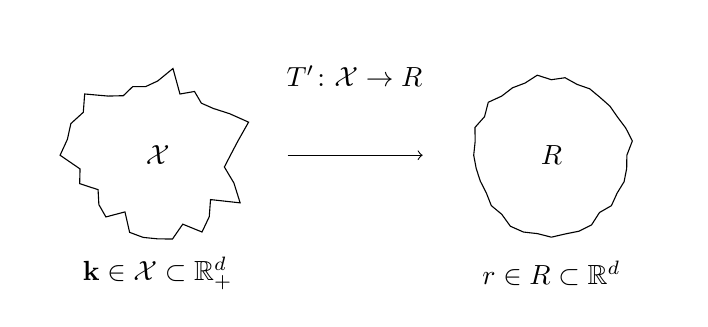
\begin{tikzpicture}
		\pgfmathsetseed{1}

		\node[inner sep=1.5cm,outer sep=0] (A) at (0,0) {$\mathcal{X}$};
		\node[inner sep=1.5cm,outer sep=0] (B) at (5,0) {$R$};

		\draw (A) \irregularcircle{1cm}{2.5mm};
		\draw (B) \irregularcircle{1cm}{0.5mm};

		\draw [->] (A) -- (B);

		\node at (2.5,1) {$T'\colon\mathcal{X}\rightarrow R$};

		\node at (0,-1.5) {$\mathbf{k}\in\mathcal{X}\subset\mathbb{R}_+^d$};
		\node at (5,-1.5) {$r\in R\subset\mathbb{R}^d$};
	\end{tikzpicture}
	\caption{Couplings between parameter space and reference when using the transport map proposal method to propose moves on parameter space.}
	\label{fig:chem_coupling}
\end{figure}

Figure~\ref{fig:chem_coupling} shows how we define a bijective map, $T'$, between parameter space $\mathcal{X}$ and a reference space $R$. In practice we cannot ensure that the approximate map $\tilde{T}'$ is uniquely invertible over the whole of $R$ and so $\tilde{T}'$ is not truly bijective. This leads to problems for our strictly positive state space, $\mathcal{X} \subset \mathbb{R}_+^d$, since proposals in $R$ do not necessarily map back on to $\mathcal{X}$. This motivates the use of a third intermediate space. When using the transport map proposal distribution, we prefix the proposal method with a T, e.g. MH-RW (RWMH) and MH-TRW, as well as PAIS-RW and PAIS-TRW.

We also consider how these algorithms perform when they are applied to the log of the reaction rates. We choose to use this log transformation since it converts our strictly positive parameter space, $\mathcal{X}$, into an intermediate space $\mathcal{Y} \subset \mathbb{R}^d$. This allows us to define $T$ between two subsets of $\mathbb{R}^d$, which means that even if $\tilde{T}$ is not uniquely invertible in some region of $R$, all possibilities are valid proposals. As before, the proposal distributions are labelled with a T for transport map and when using the intermediate space we prepend `log' to the proposal method, e.g. MH-logRW and MH-logTRW, with, PAIS-logRW and PAIS-logTRW.

\begin{figure}
	\centering
	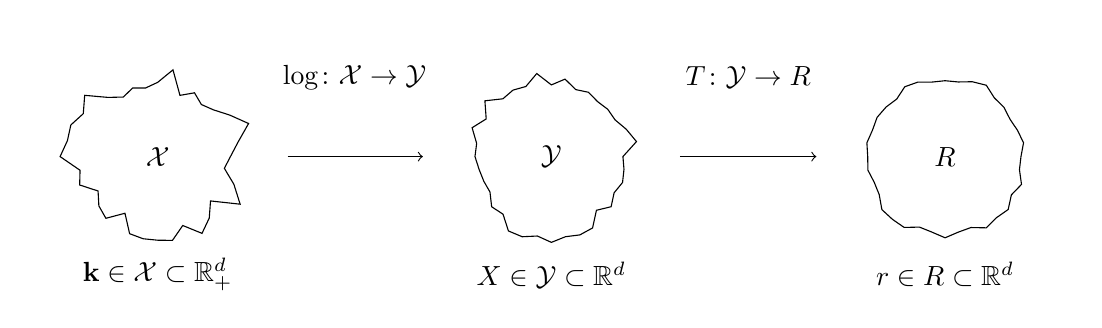
\begin{tikzpicture}
		\pgfmathsetseed{1}

		\node[inner sep=1.5cm,outer sep=0] (A) at (0,0) {$\mathcal{X}$};
		\node[inner sep=1.5cm,outer sep=0] (B) at (5,0) {$\mathcal{Y}$};
		\node[inner sep=1.5cm,outer sep=0] (C) at (10,0) {$R$};

		\draw (A) \irregularcircle{1cm}{2.5mm};
		\draw (B) \irregularcircle{1cm}{1.1mm};
		\draw (C) \irregularcircle{1cm}{0.5mm};

		\draw [->] (A) -- (B);
		\draw [->] (B) -- (C);

		\node at (2.5,1) {$\log\colon\mathcal{X}\rightarrow\mathcal{Y}$};
		\node at (7.5,1) {$T\colon\mathcal{Y}\rightarrow R$};

		\node at (0,-1.5) {$\mathbf{k}\in\mathcal{X}\subset\mathbb{R}_+^d$};
		\node at (5,-1.5) {$X\in\mathcal{Y}\subset\mathbb{R}^d$};
		\node at (10,-1.5) {$r\in R \subset\mathbb{R}^d$};
	\end{tikzpicture}
	\caption{Couplings between parameter space, an intermediate space and reference space when using the transport map proposal method to propose moves on a log space.}
	\label{fig:chem_log_coupling}
\end{figure}

Figure~\ref{fig:chem_log_coupling} displays the composition of maps when we include this intermediate space $\mathcal{Y}$. Every proposal in $R$ results in a valid proposal on $\mathcal{X}$. The inclusion of this additional map means that we must again alter our importance weight definition to reflect the pullback from $R$ through $\mathcal{Y}$. The weight is now
\[
	w_i(\theta') = \frac{\pi(\theta'|\mathbf{R},\mathbf{T})}{Q(\tilde{T}\circ\log(\theta')|\tilde{T}\circ\log(\theta^{(i-1)}))|J_{\tilde{T}\circ\log}(\theta')|},
\]
where $\theta'$ is a proposal on $\mathcal{X}$, $\theta^{(i-1)}$ is the ensemble of states from the previous iteration, and $J_{\tilde{T}\circ\log}(\theta')$ is the Jacobian of the composition of the two maps. This Jacobian is straightforward to calculate,
\[
	|J_{\tilde{T}\circ\log}(\theta')| = |J_{\tilde{T}}(\log(\theta'))||J_{\log}(\theta')|,
\]
where the first determinant is as we saw in the previous chapter, and the second is
\[
	|J_{\log}(\theta')| = \prod\limits_{i=1}^d \frac{1}{\theta'_i}.
\]

% choices made in transport map
For this problem, we continue to use monomials in each dimension in our transport map construction. We use polynomials of total order $p=4$ as the basis functions, i.e.
\[
	T_i(\theta) = \sum_{\mathbf{j}\in\mathcal{J}^{\text{TO}}_i(p)} \gamma_{i,\mathbf{j}}\psi_{\mathbf{j}}(\theta) \quad \text{where} \quad \psi_\mathbf{j}(\theta) = \prod\limits_{k=1}^i \theta_k^{j_k},
\]
and
\[
	\mathcal{J}^{\text{TO}}_i(p) = \{\mathbf{j} \in \mathbb{N}^d_0\ |\ \|\mathbf{j}\|_1 \leq p, \ \text{and}\ j_k = 0\ \forall k > i\}.
\]
Since $\mathcal{X}$ is four-dimensional, this yeilds a total of 125 map coefficients across the four index sets. This number can be reduced by using smaller index sets as discussed in~\cite{parno2014transport}.

% choice of resampler?
As with the mixture model in Section~\ref{sec:app_mixture}, we will use the AMR resampler with an ensemble size of $M=500$. This increase in ensemble size from Chapter~\ref{sec:PAIS} compensates for the increase in parameter dimension.

% analysis method
To measure the convergence of the sampling methods in this section, we will compare the convergence of the mean of each parameter. We approximate $\mathbb{E}(\mathbf{k})$ using 2.4 billion samples from the MH-RW algorithm.

%*** numerics.
\subsubsection{Convergence Analysis for the Constrained Approach to a Multiscale Chemical Reaction Model}\label{sec:chem_conv}

In this section, we demonstrate the convergence of the sample mean $\hat{\mathbf{k}}$ by approximating the relative error between the sample mean and the true mean $\mathbb{E}(\mathbf{k})$. We do this for each of the eight algorithms introduced in the previous section. Convergence is shown for the constrained approach to the multiscale system, i.e. to the posterior in Equation~\eqref{eqn:chem_QEA_posterior} with the effective degredation rate, $\hat{k}_4^{\text{CMA}}$, from Equation~\eqref{eqn:chem_CMA_rate}.

\begin{table}[!h]
\centering
\begin{tabular}{rrrrrr}
\toprule
	\multicolumn{1}{l}{Algorithm} & \multicolumn{3}{c}{MH} & \multicolumn{2}{c}{PAIS} \\ \cmidrule(lr){2-4} \cmidrule(lr){5-6}
	& & $\delta_\%$ & & $\delta_{\text{ESS}}$ & ESS \\ \midrule
	RW & & 5.5e-3 & & 1.0e-0 & 9.0e-3 \\
	TRW & & 1.2e-0 & & 4.0e-1 & 1.2e-3 \\
	logRW & & 1.7e-1 & & 1.2e-0 & 6.0e-2 \\
	logTRW & & 2.7e-2 & & 1.5e-1 & 3.5e-1 \\
\bottomrule
\end{tabular}
\caption{Optimal scaling parameters for the MH and PAIS algorithms applied to the constrained multiscale problem in Section~\ref{sec:chem_multiscale}. MH parameters optimised by acceptance rate, and PAIS parameters optimised using effective sample size.}
\label{tab:chem_multiscale_scaling}
\end{table}

The optimal scaling parameters are given in Table~\ref{tab:chem_multiscale_scaling}. We note that for MH-TRW and PAIS-TRW the scaling parameter is near to 1, particularly for MH-RW, this is what we should expect since the proposal is made on a reference space which should be near to $\mathcal{N}_d(0, \text{I})$. The same should be true for the MH-logTRW and PAIS-logTRW algorithms since these have the same target reference space, however the optimal scaling parameters here are much smaller. We see that the ESS is higher for the algorithms which sample on $\mathcal{Y}$, and we expect that convergence will be fastest for the PAIS-logTRW algorithm.

\begin{figure}[!htb]
\centering
\subfigure[Sampling algorithms on $\mathcal{X}$.]{\includegraphics[width=0.495\textwidth]{"images/CMA_L2_param_space"}}
\subfigure[Sampling algorithms on $\mathcal{Y}$.]{\includegraphics[width=0.495\textwidth]{"images/CMA_L2_log_space"}}
\caption{Convergence of the constrained multiscale example described in Section~\ref{sec:chem_multiscale}.}
\label{fig:chem_multiscale_L2}
\end{figure}

Convergence of the eight algorithms for this example is shown in Figure~\ref{fig:chem_multiscale_L2}. We first note the poor performance of the MH based algorithms, each of them taking roughly 10,000 samples to begin converging. Only the MH-TRW is at all competitive with the PAIS algorithms. During the simulation interval, the MH-TRW algorithm has not settled down to the expected $\mathcal{O}(1/\sqrt{N})$ rate which means that the estimate is still biased by the long burn-in time. As we have seen in previous examples, the burn-in time for the PAIS algorithm is negligible.

The PAIS variants with RW and TRW proposals perform similarly on both sample spaces. When sampling on $\mathcal{X}$ the transport map is not quite as efficient, largely due to the difficulties discussed in the previous section i.e. many proposals are made which do result in negative reaction rates. Sampling on $\mathcal{Y}$ leads to more comparable Monte Carlo errors, with the logTRW being apparently slightly less stable. This proposal method becomes more stable as we increase either the ensemble size, or the number of iterations between updates of the transport map, $T$. Overall we see the smallest Monte Carlo errors for a given amount of computational effort coming from the PAIS-logTRW algorithm.

\begin{figure}[!htb]
\centering
\subfigure[Reference space mapped to by $T'$.]{\includegraphics[width=0.495\textwidth]{"images/CMA_ref_space_MHTRW"}}
\subfigure[Reference space mapped to by $T\circ\log$.]{\includegraphics[width=0.495\textwidth]{"images/CMA_ref_space_MHlogTRW"}}
\caption{Reference space for the TRW and logTRW proposal distributions. Components are linked by the relation $r_i = T_i'(k_i)$ in (a) and $r_i = T_i\circ\log(k_i)$ in (b).}
\label{fig:chem_reference_spaces}
\end{figure}

We now look at the proposal distributions of the transport map accelerated algorithms. In Figure~\ref{fig:chem_reference_spaces}, we see the reference spaces found by; in (a) mapping the posterior through the map $T'$, and in (b) by mapping the posterior through $T\circ\log$. For the most part, each of these marginal distributions can be recognised as a Gaussian. However, with the exception of $\mathbb{P}(r_2,r_3)$, we would not consider them to be close to a standardised $\mathcal{N}(0, \text{I})$ distribution. Before thinking that the transport map has not helped us to find a `nicer' space on which to propose new values we should consider that the dimensions are now (1) largely uncorrelated, and (2) the variances in each dimension are much more similar than they are in Figure~\ref{fig:chem_CMA_posterior}.

Particularly in Figure~\ref{fig:chem_reference_spaces} (b) we see that $\text{var}(r_1)$ and $\text{var}(r_4)$ are much smaller than $\text{var}(r_2)$ and $\text{var}(r_3)$. To combat this we have a number of choices, we might wish to use two different scaling parameters to match these scales, which would require knowledge of the reference space before beginning sampling. We could alternatively use a proposal distribution such as in the LPAIS algorithm to adaptively learn this at each iteration. Another option is to increase the total order of our index set. For these numerics we have chosen $p=4$, but we know that we can obtain reference spaces which are closer to $\mathcal{N}_d(0, \text{I})$ by choosing a larger $p$.

\subsubsection{Comparison of the Constrained and QEA approaches}

The convergence analysis has been performed for the constrained approach to this multiscale system. We now look at the differences between the constrained and QEA posterior distributions. Recall that the approaches differed only in the form of the effective degradation rate $\hat{k}_4$,
\[
	\hat{k}_4^{\text{QEA}}(s) = \frac{k_2k_4s}{k_2+k_3} \quad \text{and} \quad \hat{k}_4^{\text{CMA}}(s) = \frac{k_2k_4s}{k_2+k_3+k_4}.
\]
This difference in the denominator causes a shift in the parameters as can be seen in Figure~\ref{fig:chem_diff}. The figure shows the difference in posteriors,
\begin{equation}\label{eqn:chem_diff}
	\text{diff}(\mu^{\text{CMA}}, \mu^{\text{QEA}}) = \pi^{\text{CMA}}(\mathbf{k}|\mathbf{R},\mathbf{T}) - \pi^{\text{QEA}}(\mathbf{k}|\mathbf{R},\mathbf{T}).
\end{equation}

\begin{figure}[htb]
\centering
\includegraphics[width=0.9\textwidth]{"images/Diff_CMA_QEA"}
\caption{Difference between the CMA and QEA posteriors as defined in Equation~\eqref{eqn:chem_diff}.}
\label{fig:chem_diff}
\end{figure}

Since the two posteriors have been approximated using an MCMC sample, there is a significant amount of noise, particularly in the tails of the distributions We can see that the differences in the marginals for $k_1, k_2,$ and $k_3$ are relatively small and the differences are largely positive. This means that the constrained approach is slightly more informative about the values of these first three parameters. However the maginal for $k_4$ varies by a significant amount and is more negative. This means that the mean estimates for $k_4$ vary by a large amount, and we should be more confident in the solution given by the QEA.

% compare solution with full data.
We now consider how we should interpret the information given by these models. The QEA assumption tells us that we cannot observe the parameters $k_2$, $k_3$ and $k_4$ indendently from the reduced data set, but we can observe the quantity $\hat{k}_4^{\text{QEA}} = k_2k_4/(k_2+k_3)$. Similarly, the constrained approach tells us that we are able to observe the quantity $\hat{k}_4^{\text{CMA}} = k_2k_4/(k_2+k_3+k_4)$. To validate our inferences on $k_2$, $k_3$ and $k_4$ we would like to discover which model is most informative about these parameters, and which model gives us results which are most similar to what we can obtain from the full model.

A conventional way to compare two models under a Bayesian framework is to calculate the Bayes factors~\cite{chen2012monte}. The Bayes factor, $B_{1,2}$, between two models, $\mathcal{M}_1$ and $\mathcal{M}_2$, can be interpreted as a ratio of the normalisation constants of the posterior distributions given each model,
\[
	B_{1,2} = \frac{\mathbb{P}(D|\mathcal{M}_1)}{\mathbb{P}(D|\mathcal{M}_2)}, \quad \text{where} \quad \mathbb{P}(D|\mathcal{M}_k) = \int_\mathcal{X} \mathbb{P}(D|\theta_k,\mathcal{M}_k)\mathbb{P}(\theta_k|\mathcal{M}_k) \, \text{d}\theta_k.
\]
Under the PAIS framework, it is straightforward to calculate these factors using the Monte Carlo estimator for the normalisation constants. From~\cite{robert2013monte} these normalisation constants take the form
\[
	Z_k \approx \frac{1}{NM}\sum_{i=1}^N\sum_{j=1}^M w_j^{(i)}(\mathcal{M}_k),
\]
where $w_j^{(i)}(\mathcal{M}_k)$ is the weight under model $\mathcal{M}_k$ corresponding to the $j$-th ensemble member on the $i$-th iteration. Hence, $B_{1,2} = Z_1/Z_2$. We can compare more than two models in this way by selecting the model with the largest marginal distribution as the best model.

We now label the constrained model as $\mathcal{M}_1$, the model arising from the QEA as $\mathcal{M}_2$, and the full data model as $\mathcal{M}_0$. Under $\mathcal{M}_1$, the parameter $\theta_1 = (k_1, \hat{k}_4^{\text{CMA}})^\top$, and under $\mathcal{M}_2$, the parameter $\theta_2 = (k_1, \hat{k}_4^{\text{QEA}})^\top$. The full model $\mathcal{M}_0$ observes all four parameters $\theta_0 = (k_1, k_2, k_3, k_4)^\top$. The marginal densities for the data, evaluated at the observed data, given the models are displayed in Table~\ref{tab:chem_Bayes_marginals}.

\begin{table}[!htb]
\centering
\begin{tabular}{rr}
	\toprule
	$k$ & \quad $\mathbb{P}(D = (\mathbf{R},\mathbf{T})^\top|\mathcal{M}_k)$ \\ \cmidrule(lr){1-2}
	0 & 6.8e-3 \\
	1 & 3.2e-3 \\
	2 & 1.7e-3 \\ \bottomrule
\end{tabular}
\caption{Marginal distributions for the data $(\mathbf{R},\mathbf{T})^\top$ for each model considered in Section~\ref{sec:multiscale_posterior}.}
\label{tab:chem_Bayes_marginals}
\end{table}

Computing the Bayes factors from Table~\ref{tab:chem_Bayes_marginals} we see that we should of course prefer the model in which we observe all reactions perfectly, however this model is not significantly better than the CMA model ($B_{0,1} = 2.09 < 3.2$, ~\cite{kass1995bayes}). Again the constrained model is not substantially more attractive than the QEA model when we consider the Bayes factor $B_{1,2} = 1.96 < 3.2$. The Bayes factor $B_{0,2} = 4.1 > 3.2$ does tell us that we should significantly prefer the full model to the QEA model. These Bayes factors present a weak argument that that the constrained model provides us with a better description of the data than the QEA model. We can also present this information graphically, which might provide us with a greater justification for preferring the constrained model.

\begin{figure}[!htb]
\centering
\subfigure[Marginal for $\hat{k}_4^{\text{QEA}}$.]{\includegraphics[width=0.495\textwidth]{"images/QEA_approx_marginal"}}
\subfigure[Marginal for $\hat{k}_4^{\text{CMA}}$.]{\includegraphics[width=0.495\textwidth]{"images/CMA_approx_marginal"}}
\caption{Comparison of the approximate marginal densities for the `observable parameter' $\hat{k}_4$ under models $\mathcal{M}_1$ and $\mathcal{M}_2$. Marginals for these two parameters are approximated using samples which have been produced by targeting the three densities $\pi_i = \mathbb{P}(\theta_i|D,\mathcal{M}_i)$ for $i = 0, 1, 2$.}
\label{fig:chem_model_comp}
\end{figure}

Figure~\ref{fig:chem_model_comp} displays the marginal distributions for the parameters $\hat{k}_4^{\text{QEA}}$ and $\hat{k}_4^{\text{CMA}}$. For each of these two observable parameters we obtain approximations for three marginal distributions, $\pi_i(\cdot|D, \mathcal{M}_i)$, $i = 0, 1, 2$. Each of these approximations has been produced by marginalising a sample drawn from the full posterior $\pi_i(\mathbf{k}|D, \mathcal{M}_i)$ defined in terms of the respective model $\mathcal{M}_i$. In other words, to calculate $\hat{\pi}_1(\hat{k}_4^{\text{QEA}}|D)$, we first draw a sample using the PAIS algorithm targeting the posterior density $\pi_1(\mathbf{k}|D,\mathcal{M}_1)$. We then calculate $\theta^{(j)} = k_2^{(j)}k_4^{(j)}/(k_2^{(j)}+k_3^{(j)})$ for each sample produced. Finally we produce a histogram from this sample $\theta^{(j)}$.

The first thing to note is that in subfigure (a) when we approximate the marginals for $\hat{k}_4^{\text{QEA}}$ the density $\hat{\pi}_2(\cdot|D,\mathcal{M}_2)$ is much more peaked than $\hat{\pi}_1(\cdot|D,\mathcal{M}_1)$. As we might expect the same is true in reverse in subfigure (b). What is interesting here is that for both parameters, the marginal distribution which assumes $\mathcal{M}_2$ assigns a small density value to the true value of the parameter, while the marginals which assume $\mathcal{M}_1$ assign a relatively high density to the truth. We also draw attention to the similarities between the constrained model and the full data model. In subfigure (a) these two marginals are peaked around a similar value, and in subfigure (b) the full data and constrained models almost exactly coincide. This supports the hypothesis that the constrained approach provides a more accurate approximation to the dynamics of the full system.

\section{Conclusions}\label{sec:conc}

\bibliographystyle{siam}
\bibliography{refs}
\end{document}
